In this chapter we will introduce the basic principles required to understand what waveplates are and how they work in general. Simply put the purpose of a waveplate is to change the polarization of EM waves, most commonly by using a birefringent material. The polarization of EM waves, birefringence and how the waveplates work are explained in more detail in the sections \ref{sec:polellipse}, \ref{sec:birefringence} and \ref{sec:waveplates}. This change of the polarization state caused by the waveplate, and the state itself, can be described mathematically using Jones calculus or almost equivalently using Mueller calculus, which will be shown in section \ref{sec:mathdescription}. Finally, this leads to the description of the design and the design optimization problem in the last section (\ref{sec:design}) of this chapter.


\section{The polarization ellipse}
\label{sec:polellipse}
There are several ways to describe the polarization state of EM-waves. One of them is the polarization ellipse which is a geometrical representation of the polarization. This remained the only satisfactory way to visualize the different polarization states for almost the entire 19\textsuperscript{th} century, although it is not very practical for carrying out calculations. At the end of the century another representation was proposed by Henri Poincaré, now known as the Poincaré sphere, which could be used for both calculations and visualization of the polarization states \cite{Collett2008VisualizationSphere}. Poincaré's representation will be explained in section \ref{sec:muellercalc}. The polarization ellipse can be derived either directly from a solution to the EM-wave equation or starting from Maxwell's equations.  It is practical to start from Maxwell's equations, since they are used for derivations later on in this work and almost all equations used originate from them. In differential form Maxwell's equations are given by: 
\par
\noindent\begin{minipage}{.5\linewidth}
\begin{align}
    \bm{\nabla}\cdot\bm{D} &=\rho_{f}\;,\label{eq:maxwell1}
    \vphantom{\frac{\partial\bm{B}}{\partial t}}\\
    \bm{\nabla}\cdot\bm{B} &=0\;,\vphantom{\frac{\partial\bm{B}}{\partial t}}\label{eq:maxwell2}
\end{align}
\end{minipage}%
\begin{minipage}{.5\linewidth}
\begin{align}
    \bm{\nabla}\times\bm{E} &=-\frac{\partial\bm{B}}{\partial t}\;,\label{eq:maxwell3}
    \\
    \bm{\nabla}\times\bm{H} &=\bm{J}_f
    +\frac{\partial\bm{D}}{\partial t}\;,\label{eq:maxwell4}
\end{align}
\end{minipage}
\newline

where $\bm{E}, \bm{H}$ denote the electric and magnetizing fields respectively,  $\bm{D}=\hat{\epsilon} \bm{E}$ is the electric displacement, t is the time and $\hat{\epsilon}$ is the permittivity, which depends on the material and is a complex function of the frequency. The materials used in this work are non magnetic, which means that the magnetic and magnetizing fields are proportional: $\bm{B} = \mu_0 \bm{H}$, where $\mu_0$ denotes the vacuum permeability. $\rho_f, \bm{J}_f$ is the free charge and current density respectively. Usually in optics there are no free charge carriers or free currents, which is also the case for all materials in this work, so we set $\rho_f=\bm{J}_f=0$ \cite{Roth2019Optik}. If we then also assume that the materials are homogeneous so that $\hat{\epsilon}$ does not depend on position, then we can reduce equations \ref{eq:maxwell1}-\ref{eq:maxwell4} to the following:

\noindent\begin{minipage}{.5\linewidth}
\begin{align}
    \bm{\nabla}\cdot \bm{E} &=0\;,\label{eq:maxwell1reduced}
    \vphantom{\frac{\partial\bm{B}}{\partial t}}\\
    \bm{\nabla}\cdot\bm{B} &=0\;,\vphantom{\frac{\partial\bm{B}}{\partial t}}\label{eq:maxwell2reduced}
\end{align}
\end{minipage}%
\begin{minipage}{.5\linewidth}
\begin{align}
    \bm{\nabla}\times\bm{E} &=-\frac{\partial\bm{B}}{\partial t}\;,\label{eq:maxwell3reduced}
    \\
    \bm{\nabla}\times\bm{B} &=\mu_0 \hat{\epsilon} \frac{\partial\bm{E}}{\partial t}\;,\label{eq:maxwell4reduced}
\end{align}
\end{minipage}
\newline

Applying $\bm{\nabla}\times$ to equation \ref{eq:maxwell3reduced} and with equation \ref{eq:maxwell4reduced} we decouple $\bm{E}$ and $\bm{B}$: 
\begin{equation}
    \bm{\nabla}\times \bm{\nabla}\times \bm{E} = -\mu_0 \hat{\epsilon} \frac{\partial^2\bm{E}}{\partial t^2}
\end{equation}
Then using the vector calculus identity: $\bm{\nabla}\times \bm{\nabla}\times \bm{F} = \bm{\nabla} \left( \bm{\nabla} \cdot \bm{F} \right) - \bm{\nabla}^2 \bm{F}$, for any function $\bm{F}$, together with equation \ref{eq:maxwell1reduced} we get the EM-wave equation: \footnote{We neglect the magnetic field, since we are only concerned with non magnetic materials in this work. But the derivation of the wave equation for the magnetic field would be exactly the same}
\begin{equation}
    \label{eq:waveeq}
    \bm{\nabla}^2 \bm{E} = \mu_0 \hat{\epsilon} \frac{\partial^2\bm{E}}{\partial t^2}
\end{equation}
and via a Fourier transform $(\partial_t \xrightarrow{\mathscr{F}} i\omega)$ we readily get the Helmholtz equation for $\bm{E}$:
\begin{equation}
    \label{eq:waveeqfreq}
    \bm{\nabla}^2 \bm{E} = -\mu_0 \hat{\epsilon} \omega^2 \bm{E},
\end{equation}
where $\omega$ is the angular frequency.
A solution to the wave equation is a coherent plane wave at frequency $\omega$ which is given by: 
\begin{equation}
    \label{eq:planewave}
    \bm{E} = \bm{E_0} e^{i(\bm{k}\bm{r} - \omega t + \delta)},
\end{equation}
where $\bm{r}$ and $\bm{k}$ denote the position and wave vector respectively, $\bm{E_0}$ denotes the maximum amplitude of the wave and $\delta$ is the phase constant. If we assume the wave propagates along the z-direction in a Cartesian coordinate system, then the amplitude will be orthogonal to the z-direction, i.e a transverse wave. This follows directly from equation \ref{eq:maxwell1reduced}. From the wave equation in frequency space we then find the requirement that the wave number, which is the magnitude of the wave vector, and the angular frequency are related by:
\begin{equation}
    \label{eq:wavevector_req}
    k = \sqrt{\mu_0 \hat{\epsilon}} \omega
\end{equation}
The phase velocity of the wave can then be expressed as:
\begin{equation}
    v = \frac{\omega}{k} = \frac{1}{\sqrt{\mu_0 \hat{\epsilon}}} = \frac{c}{\tilde{n}},\:\tilde{n} = \sqrt{\frac{\hat{\epsilon}}{\epsilon_0}},
\end{equation}
where $c$, $\epsilon_0$ and $n$ is the speed of light in vacuum, vacuum permittivity and refractive index respectively.
So that from the wave equation we get two decoupled wave equations, each describing an oscillation in the x-z plane and the y-z plane. This is also known as Fresnel's wave theory which was proposed and verified experimentally around 1820 by Augustin-Jean Fresnel and François Arago, more than 40 years before Maxwell's equations were published \cite{Collett2009FieldPolarization,Jackson1998ClassicalEdition}.
This means equation \ref{eq:planewave} consists of only two perpendicular components. Additionally, if we consider that Maxwell's equations \ref{eq:maxwell1reduced}-\ref{eq:maxwell4reduced} are all linear and real, then it follows that the real part of any particular solution is also a solution to the wave equation. \footnote{This only works if the equations are real. For example, Schrödinger's equation is linear but complex, therefore even if $\psi$ is a solution $\operatorname{Re}(\psi)$ and $\operatorname{Im}(\psi)$ are not.} We can then write equation \ref{eq:planewave} as two sinusoidal waves:
\begin{equation}
\label{eq:plane_wave_realparts}
\begin{aligned}
    E_x(z, t) = E_{0x}\cos(kz-\omega t + \delta_x) \\
    E_y(z, t) = E_{0y}\cos(kz-\omega t + \delta_y), 
\end{aligned}
\end{equation}
where $\delta_x$ and $\delta_y$ are arbitrary phases of the two components. Depending on the values of $E_{0x}, E_{0y}$ and the relative phase or simply phase, which is $\delta = \delta_y - \delta_x$, we get different polarization states. Figure \ref{fig:Ex_Ey_planewaves} shows the real parts of the two plane wave components for a wave traveling along the z-direction when $\delta=0$ and $E_{0x}=E_{0y}$.

\begin{figure}[h]
    \centering
    \includestandalone{3_chapter03/tikz_e_wave}
    \caption{This figure shows the two sinusoidal waves given in equation \ref{eq:plane_wave_realparts}, which are the real parts of the plane wave components. Both waves have the same amplitude and phase.}
    \label{fig:Ex_Ey_planewaves}
\end{figure}

From here we can visualize the different polarization states, that is the different directions the electrical field, or simply the light, can oscillate in. If the light is confined to a plane along the direction of propagation it is said to be linearly polarized (LP). An example of this is shown in figure \ref{fig:E_planewave}, where the polarization plane is at an angle of \SI{45}{\degree} relative to the x-axis. 

\begin{figure}[h]
    \centering
    \includestandalone[scale=1.1]{3_chapter03/tikz_linear_pol}
    \caption{The black curve shows the superposition of the two sinusoidal waves from equation \ref{eq:plane_wave_realparts}, which is the same as the real part of a LP plane wave at an angle of \SI{45}{\degree} to the x-axis. In addition, the horizontal and the vertical components of the field vector are shown as the red and blue curves respectively.}
    \label{fig:E_planewave}
\end{figure}

Now, if $\delta$ is exactly $\nicefrac{\pi}{2}$ and $E_{0x} = E_{0y}$, then we get the case shown to the right in figure \ref{fig:circ_pol_planewave}. A field with this kind of polarization traces out a circle as time passes for a fixed position in space. On the other hand, if we keep time fixed then the field vector describes a helix along the direction of propagation. This means the field only changes direction but not its magnitude. This type of polarization is therefore called circular polarization (CP). Additionally, because we can trace out a circle in two different directions (clockwise or counterclockwise) we therefore get two different types of circular polarizations. These two types are called right CP (RCP) or left CP (LCP) depending on the direction the circle is traced out, so either in a left- or right-handed sense. This is called the handedness of the light, which can be determined using the right hand rule. For that we fix the right hand at a point on the helix and point the thumb away from the receiver, that is against the direction of propagation. Then the light is right-handed if the helix is traced out in the direction of the other fingers as time revolves, otherwise it is left-handed. The light shown to the left of figure \ref{fig:circ_pol_planewave} is therefore left-handed while the example on the right side of figure \ref{fig:circ_pol_planewave} shows right-handed CP light. The reason why we have two types of CP in the first place, is because of the fact that one component can lead the other, as we can see in figure \ref{fig:circ_pol_planewave}. Where for RCP the horizontal component leads the vertical one by a quarter period ($\delta = -\nicefrac{\pi}{2}$), for LCP it is the other way around and $\delta = \nicefrac{\pi}{2}$. 

\begin{figure}[h]
\centering
    \begin{subfigure}
        \centering
        \includestandalone[scale=0.8]{3_chapter03/tikz_circ_pol_lh}
    \end{subfigure}
    \begin{subfigure}
        \centering
        \includestandalone[scale=0.8]{3_chapter03/tikz_circ_pol_rh}
    \end{subfigure}
    \caption{The left figure shows an example of LCP light and the right figure RCP light. Furthermore, handedness originates from one component leading the other. In the case of LCP light the vertical component leads the horizontal component and vice versa for RCP light.}
    \label{fig:circ_pol_planewave}
\end{figure}

Finally, the last polarization state we have not mentioned yet, even though it is in fact the most general, is the elliptical polarization state. The polarization states we have dealt with so far have all been limiting cases of this state. For a fixed position this is fairly simple to visualize geometrically; LP light traces out a line while CP light traces out a circle, both of these shapes are degenerate forms of an ellipse. A summary of the different degenerate states and the corresponding amplitude and phase combinations are shown in table \ref{tab:pol_state_summary}, which is divided into three parts with a pair of states in each. At the top there str the linear horizontal/vertical polarization (LHP/LVP) stated, the linear $\pm\SI{45}{\degree}$ polarization ($L_{\pm45}P$) states are in the middle and the CP states are at the bottom. The last column shows the corresponding degenerate ellipse for each state.

\begin{table}
    \centering
    \includestandalone{3_chapter03/pol_summary_table}
    \caption{Summary of the different degenerate polarization states, with corresponding conditions figures. The first four states are linearly polarized at different angles relative to the x-axis; $\SI{0}{\degree}$, $\SI{90}{\degree}$, $\SI{45}{\degree}$ and $\SI{-45}{\degree}$ respectively. The last two are the RCP and LCP states.}
    \label{tab:pol_state_summary}
\end{table}

We can also realize this mathematically by eliminating the time and position dependency of the two components in equation \ref{fig:Ex_Ey_planewaves}, so that we get \footnote{The derivation is given in \ref{sec:deriv_pol_ellipse}}:

\begin{equation}
    \centering
    \frac{1}{\sin^2 \delta} \left[ \left(\frac{E_x}{E_{0x}}\right)^2+\left(\frac{E_y}{E_{0y}}\right)^2-2\frac{E_x E_y}{E_{0x} E_{0y}}\cos \delta \right]=1,
\end{equation}

which describes an ellipse in its nonstandard form. Because of this the equation is called the polarization ellipse. It is worth noting that even though the time and position dependencies have been explicitly eliminated, the wave components $E_x$ and $E_y$ continue to depend on them. That means $E_{0x}$, $E_{0y}$ and $\delta$ are the polarization ellipse parameters, which then define the shape of the ellipse. Therefore, even though the light propagates the shape remains constant. There are several ways to parameterize the polarization ellipse or ellipses in general using two variables. One way is to use the ellipticity angle $\chi$ and the orientation angle $\psi$, which both can be expressed through the polarization ellipse parameters: 

\begin{equation}
    \tan 2\psi = \frac{2E_{0x}E_{0y}}{E_{0x}^2 - E_{0y}^2}\cos \delta,\: 0\leqslant\psi\leqslant\pi,
\end{equation}
\begin{equation}
    \sin 2\chi = \frac{2E_{0x}E_{0y}}{E_{0x}^2 + E_{0y}^2}\sin \delta,\: \nicefrac{-\pi}{4}\leqslant\chi\leqslant\nicefrac{\pi}{4}.
\end{equation}
Figure \ref{fig:pol_ellipse} shows an example of a polarization ellipse together with the orientation and ellipticity angles. We see from the figure that for $\psi \rightarrow 0/\pi$ or $\psi \rightarrow \nicefrac{pi}{2}$ the major and minor axes $(a$ and $b)$ coincide with the coordinate axes. Likewise for $\chi \rightarrow 0$ the ellipse degenerates to a line and for $\chi \rightarrow \pm\nicefrac{\pi}{4}$ we get a circle \cite{Collett2009FieldPolarization}.

\begin{figure}[h]
    \centering
    \includestandalone{3_chapter03/tikz_pol_ellipse}
    \caption{Example of a polarization ellipse, which shows the ellipticity and orientation angle geometrically. The major and minor axes of the polarization ellipse are denoted by $a$ and $b$ respectively. We see that $\chi$ changes with the shape of the ellipse while $\psi$ is simply the orientation relative to the x-axis.}
    \label{fig:pol_ellipse}
\end{figure}

We finish off this section, as a bit of a side note, by mentioning the conventions used so far. If we go back to the plane wave solution (equation \ref{eq:planewave}) of the wave equation we see that a replacement of $i$ with $-i$ yields another valid linearly independent solution. This leads to two different sets of definitions, depending on the of the imaginary unit. The first one, with a positive sign and the one used here, is commonly used in physics texts. While the other one with a negative sign is mainly used in electrical engineering (EE) texts. Mathematically the difference between these two conventions is simply the direction of rotation of the phasor in the complex plane with increasing time. An example of this is shown for a phasor $x$ in figure \ref{fig:phasor}. 

\begin{figure}[h]
    \centering
    \includestandalone[scale=1.25]{3_chapter03/tikz_phasor_rotation}
    \caption{Example of a phasor $x$ in the complex plane. The sign of the imaginary unit determines the direction of rotation for increasing times. The rotation is indicated by the blue arrows and is either in the clockwise $(-i)$ or counterclockwise $(+i)$ direction.}
    \label{fig:phasor}
\end{figure}

The choice of sign has other implications. We know from equation \ref{eq:wavevector_req} that the wavevector is in general complex because the permittivity is, so we can write it as $k=\beta + i \alpha$. On the other hand we get two expressions for a plane wave propagating in the z-direction, one for each definition:
\begin{align}
    &\bm{E_{0}}e^{i((\beta + i \alpha)z-\omega t + \delta)} \\
    &\bm{E_{0}}e^{-i((\beta + i \alpha)z-\omega t + \delta)}, 
\end{align}
if we factor out the $\alpha$ dependency we get:
\begin{align}
    e^{-\alpha z}&\bm{E_{0}}e^{i(\beta z-\omega t + \delta)} \\
    e^{\alpha z}&\bm{E_{0}}e^{-i(\beta z-\omega t + \delta)}. 
\end{align}
We see that in case of the EE definition the amplitude would increase as the wave propagates, which is nonsense.\footnote{This problem also arises in the derivation of the Lorentz oscillator model. More about this in the appendix (section \ref{sec:lorentz_model_sign}), since it is out of scope of this work.} Therefore the sign of the imaginary part of the wavevector must be chosen accordingly. So for the EE definition we get:
\begin{equation}
    k=\beta - i \alpha
\end{equation}
and 
\begin{equation}
    k=\beta + i \alpha
\end{equation}
for the physics definition.
As a result the sign of the imaginary part of the refractive index will also depend on the chosen definition. When the EE definition is used:
\begin{equation}
    \tilde{n}= n - i \kappa
\end{equation}
and using the physics definition:  
\begin{equation}
    \tilde{n}= n + i \kappa
\end{equation}

The physics definition is used for example in the textbooks by John D. Jackson \cite{Jackson1998ClassicalEdition} and David J. Griffiths \cite{Griffiths2017IntroductionElectrodynamics} and also in \cite{Collett2009FieldPolarization}, which is the reference used for most of this section.
There are not only convention differences between engineers and physicists but also even between different branches of physics. The definition of CP handedness relies on the point of view; that is either looking from the source in the direction of propagation or from the receiver against the direction of propagation. Here we use the version which is defined from the point of view of the receiver. This is also the convention commonly used in optics \cite{Bass2016HandbookOptics, M.LandiDeglInnocenti2004PolarizationLines} as well as by SPIE \cite{Collett2009FieldPolarization}.
The other convention is used by radio astronomers \cite{1973CommissionAstronomie}, quantum physicists, because it is consistent with the convention of handedness for a particle's spin and it is also used by electrical engineers \cite{Orfanidis2004ElectromagneticAntennas}.

\section{polarization change or something}

In the previous section we saw that the electrical field consists of two components which trace out an ellipse as time propagates for a fixed position. Additionally, the shape and orientation of the ellipse depends on the relative phase of the two components as well as their amplitudes. Naturally this dependency is symmetrical in the two amplitudes and the relative phase. Therefore in order to change the polarization state, the change in each of the individual phases must be different and or that of the two amplitudes. 
Materials with a direction dependent absorption are said to be dichroic, e.g. the amplitudes will vary differently for a wave propagating in such a material.
This can happen if the wave propagates in a dichroic material, that is a material where the absorption is direction dependent. Then the magnitude of the amplitude will vary differently. 
Consequently, for this to happen the medium the wave is propagating in must be anisotropic. the property of a material to be absorping 
If the absorption of a material is direction dependent then the material is dichroic, e.g the amplitudes change will be different between the two components

Add E perp to K and B etc. in beginning of maxwell stuff...
maybe add small note about why dealing with single frequency makes sense -> fft, superposition principle stuff (griffiths explains it 7.12 or something)

two main effects that change polarization why? stuff do intro -> birefringence, dichroism phenomelogical -> explanation optics by eugene 351
indexellipsoid.

\subsection{Dichroism}


\subsection{Birefringence}
\label{sec:birefringence}
Birefringence is the material property responsible for the phenomenon of double refraction. This phenomenon was observed for the first time in calcite crystals by the Danish scientist Rasmus Bartholin in 1669 \cite{RasmusBartholin1669ExperimentaDetegitur, Restaino2015PolarizationDevices}. The effect of double refraction on a light beam passing through a birefringent material is relatively easy to show. One can simply place a birefringent crystal on top of some text, as it is shown in figure \ref{fig:3birefringence}. Two images of the text become visible through the crystal and each image is shifted by a different amount. These images are not simply reflections at the crystal-air interface, since the images are brighter compared to images formed through reflections, and they are even visible when looking down directly from above. Also if the crystal is rotated then one of the pictures will be stationary, while the other one will circle around the stationary image. The same effect can be illustrated by sending an unpolarized laser beam through the crystal. The beam is split in two as it propagates through the crystal. Another effect of birefringence, which is more subtle, is that each of the two beams exiting the crystal will be polarized perpendicular to each other \cite{Roth2019Optik}.

\begin{figure}[h]
    \centering
    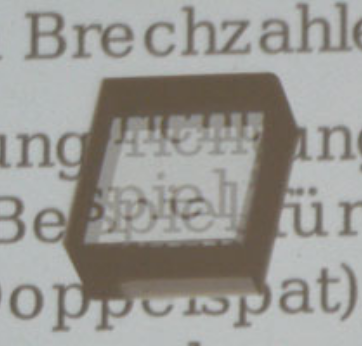
\includegraphics[scale=0.35]{images/3_chapter03/birefringence.png}
    \caption{A calcite crystal placed on top of some text. This demonstrates the effect of birefringence on the original image seen through the crystal. \cite{Roth2019Optik}}
    \label{fig:3birefringence}
\end{figure}

The underlying cause of birefringence can be explained by considering the structure of the material. In birefringent 

\subsection{Natural}

\subsection{Form birefringence}

\section{Waveplates}
\label{sec:waveplates}

\section{Mathematical description}
\label{sec:mathdescription}

\subsection{Boundary conditions}

\subsection{Jones calculus}

\subsection{Mueller calculus}
\label{sec:muellercalc}

\section{Design description}
\label{sec:design}

\subsection{Optimization?}
- describe algorithm
